\documentclass[twocolumn]{article}
\usepackage{array,url,kantlipsum}
\usepackage{lineno,hyperref}
\usepackage{graphicx}
\usepackage{float}
\graphicspath{{./Figures/}}

\begin{document}
\twocolumn[{%
 \centering
 \LARGE Fool-Proofing Recipe Measurements \\[0.5em]
 \large By Samantha Maticka and Kurt Nelson \\[1em]
 \normalsize
}]

\begin{abstract}
This text should be back in two columns
\end{abstract}

\section{Introduction}
Many of us casual cooks are not able to reproduce winning recipes when applying the Italian Grandma method (IGM), and instead we are left with one-hit-wonders followed by an onslaught of failed recreation attempts that pale in comparison and litter your fridge with dreadful leftovers. Our project seeks to end this dystopia. 

The broader objective of our project is to create a smart recipe recorder and instructor. Essentially, you can either 1) make a recipe-free dish, in which you add ingredients at will and a smart device films and records the recipe, or 2) you can create a saved recipe, where the device tells you when to stop pouring a specified ingredients. 
 	
We therefore propose applying machine learning and computer vision to teach phones how to measure for us. As a first step to solving this burdensome problem, our project will focus on volume prediction of a poured liquid. The world will soon be a better place.

\section{Goal}     
Given features about a flowing liquid, one can calculate the volume poured with basic principles. Namely 
\begin{equation} \label{eq:1}
V = \int v(t,z) A(t,z) dt \\,
\end{equation}
where $V$ is the total poured volume, $v(t,z)$ is the velocity of the pour stream, and $A(t,z)$ is the stream area. $v(t,z)$ and $A(t,z)$ are both time dependent and require evaluation at a fixed reference height $z$. However the calculation can be simplified if the a representative time average area $\overline{A}$ and velocity $\overline{v}$ are known over a pour duration $\overline{T}$, giving $V = \overline{A} \overline{v} \overline{T}$. Each of these features can be extracted from footage of liquid being poured using computer vision techniques. However, due to our crude estimate of a time-varying process this prediction method has error. The idea of using machine learning to estimate volume is to improve the accuracy of our volume prediction. 

\section{Experiments}
To create our data, we filmed over 100 videos of liquid being poured into a bowl (~10 video samples per volume, with volumes ranging from 1/4 cups (c) to 2 1/4 c, in 1/4 c increments). The experiments were kept highly controlled to minimize error resulting from the setup; we used blue water to enhance contrast, chose a setup that minimized glare and shadowing, and included a ruler to calibrate pixel lengths. 

\section{Features and labels}
To process the videos, each film was broken into a series of still frames. Based on the contrast of consecutive image intensities, the frames were used to find the start and stop times of the poured liquid (Figure ??), which was then used to estimate the pour duration. The area was predicted from each video by first identifying the stream width at different heights based on red color intensity variations (Figure ??), which was then squared and averaged to compute the mean area. Velocity was estimated by tracking the front of the falling liquid using edge detection. After processing predictions of $\overline{A}$, $\overline{v}$, and $\overline{T}$ were extracted. We checked to see how each of the features correlated to the known poured volume ($y$) and the other 2 features.

\section{Machine learning}
\subsection{Ordinary least squares feature selection}
Forward search was applied to identify relevant features for the ordinary least squares (OLS) fit. The original features ($\overline{A}$, $\overline{v}$, and $\overline{T}$), all 2nd order terms ($\overline{A}^2$, $\overline{v}^2$, and $\overline{T}^2$), and 4 interaction terms ($\overline{T} \overline{v}$, $\overline{T} \overline{A}$, $\overline{A} \overline{v}$, and $\overline{T} \overline{A} \overline{v}$) were considered. As features were sequentially added to the model, leave-one-out cross validation (LOOCV) was applied to identify the feature at each step that reduced the generalize cross validation error ($CV$) the most. Here, $CV$ is defined as
\begin{equation} \label{eq:2}
CV = \frac{1}{m} \sum^{m}_{i=1} \left( y^{(i)}-h^{(i)}_{OLS} \right)^{2} \\,
\end{equation}
where $h^{(i)}_{OLS}$ is the model prediction of $y^{(i)}$ at $x^{(i)}$ from an OLS fit using all observation but $x^{(i)}$. The generalized cross validation error is shown as a function of the number of model features in Figure \ref{fig:CVerror}. 

\begin{figure}
\centering
 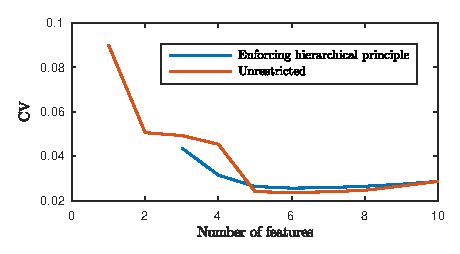
\includegraphics[width=80mm]{featureSelection}
 \caption{CV error from forward search with LOOCV as a function of feature numbers for an unrestricted search, and a search obeying the hierarchical principle}
 \label{fig:CVerror}
  \end{figure}
 
 Forward search was applied in two forms. In the first, no restrictions were evoked on which features were contained within the model (red line). In the second, forward search was applied while enforcing the hierarchical principle (blue line), which states that if an interaction or high order term is added to a model, then so should the main features involved (James et al. [2013]). For example, if $\overline{T} \overline{A} \overline{v}$ is added to the model, then individual terms for $\overline{T}$, $\overline{A,}$ and $\overline{v}$ must also be included. As shown in Figure 3, both forms of the forward search suggest model performance does not significantly increase using beyond five feature. However, the exact features selected depends on the restrictions applied. Enforcing the hierarchical principle selected $\overline{T}$, $\overline{A}$, $\overline{v}$, $\overline{T} \overline{A} \overline{v}$, and $\overline{A}^{2}$, while the unrestricted search identified $\overline{T} \overline{v}$,  $\overline{T} \overline{A}$, $\overline{v}$, $\overline{A}$, $\overline{A}^{2}$ as the most relevant features. We chose the 5 features identified by the hierarchical search for our ordinary least squares model. This choice was made not only to obey hierarchical principle, but also because the selected model contains $\overline{T} \overline{A} \overline{v}$ which has physical significance. 


\subsection{Physical prediction vs OLS prediction} As a baseline for comparison, volume predictions were also made assuming a physical based model 
\begin{equation} \label{eq:3}
h^{(i)}_{phy} = \alpha T^{(i)} A^{(i)} v^{(i)}\\,
\end{equation}
where $\alpha = \sum^{m}_{j=1} y^{(j)}/(T^{(j)} A^{(j)} v^{(j)})$ and hence is a constant chosen to minimizes the OLS fit for a model containing only $\overline{T} \overline{A} \overline{v}$. Physically, $\alpha$ represents a correction factor that attempts to account for errors in the extracted features and encompasses the required constant for an area prediction (i.e. includes a factor of $\pi/4$ if the cross-sectional area of the stream is truly a circle). We take $h^{(i)}_{phy}$ as the baseline estimate for the volume prediction based on purely physics. LOOCV was performed and a $CV$ error based on Equation (\ref{eq:2}) with $h^{(i)}_{phy}$ has the hypothesis was computed as 0.173. Comparing this to the 0.026 C$V$ error from the OLS model with $\overline{T}$, $\overline{A}$, $\overline{v}$, $\overline{T} \overline{A} \overline{v}$, $\overline{A}^{2}$ and bias term as features, the model identified by simple forward search reduces the $CV$ error by more than 85\%.  

\subsection{OLS Model evaluation} The 5-featured OLS model was further evaluated by investigating the dataset size affects on model performance. The original dataset was sub-sampled at different sizes, then split into 70\% training data, and 30\% test data. The mean squared error (MSE) between the predicted and actual volume was then computed for both the test and training data, and is shown in Figure \ref{fig:ModelEval}. The test and training MSE are converging, however there is currently a gap between the two. Additional data will likely improve the OLS model, and a more sophisticated model all together such as a random forest may reduce model bias and potentially reduce both the training and test MSE.

\begin{figure}
\centering
 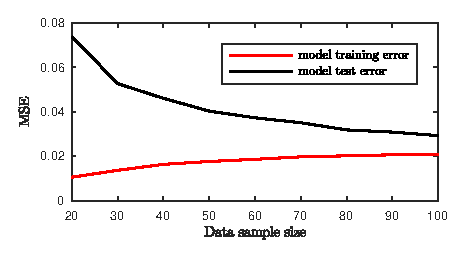
\includegraphics[width=80mm]{dataSampleSize}
 \caption{: Model and training error as a function of dataset size.}
 \label{fig:ModelEval}
 \end{figure}
\end{document}
              